\chapter{Evaluation}

\begin{figure*}
    \centering
    \small
     \begin{tabular}{l|c|r|l}
       \bf Application        & \bf Type    & \bf LoC & \bf Policies   \\
      \hline
       Atomic~\cite{atomic} (v0.34.2)       & Graph DB    & 9.6k   & Access Control                                 \\
       Contile~\cite{contile} (v1.11.0)     & Advertising & 4.9k     & Purpose Limitation                           \\
       Freedit~\cite{freedit} (v0.6.0-rc.3) & Social      & 6.6k     & Data Retention/Expiration                     \\
       Hyperswitch~\cite{hyperswitch} (v0.2.0)   & Payments    & 198.9k     & \makecell[l]{Credential Security,\\Limited Data Collection}  \\
       Lemmy~\cite{lemmy} (v0.16.6)        & Social      & 31.4k   & Access Control                               \\
       Plume~\cite{plume} (v0.7.2)         & Blogging    & 21.4k   & Data Deletion                                \\
       WebSubmit~\cite{websubmit} (v1.0)       & Homework    & 1.6k    & Data Deletion, Access Control     \\
    \end{tabular}
    \caption{Case study applications with code size and policies.}
    \label{f:apps}
   \end{figure*}

We evaluate \syslang{} against seven third-party Rust applications to answer four questions:
%
\begin{enumerate}[nosep]
    \item Can \syslang's grammar express real-world \policies? (\S\ref{sec:expressivity})
    \item How do \syslang's abstractions impact policy precision and correctness?(\S\ref{sec:precision})
    \item Are \syslang's policies efficient enough for practical use? (\S\ref{sec:efficiency})
    \item What is the effort required to encode policies in \syslang? (\S\ref{sec:accessibility})
\end{enumerate}
%

We tried to pick popular applications spanning different policy domains.
%
We summarize the applications in~\Cref{f:apps}.

\section{Expressivity}
\label{sec:expressivity}
%
We found that \syslang{} could express all of the policies that we defined for these applications.
%
In cases where the policy was inherently dynamic, we defined static approximations.
%
For example, a GDPR data deletion policy would state that some \controller{} deletes \emph{all} of a user's data.
%
\sys{} cannot verify that the application actually deletes all of the user's data,
since the exact contents of that data are only known at runtime.
%
However, it can ensure that for each type marked \lstinline[language=CNL]|@@user_data@@|, 
there is some data of that type that goes to a \lstinline[language=CNL]|"deleter"|.
%
This policy is expressive enough to find bugs where applications forget to delete a given type of user data,
but cannot catch bugs where an application only deletes \emph{some} of the data of a given type.
%

While we were able to express all of the policies for these applications,
\syslang{} has limitations that prevent it from expressing every privacy policy.
%
For example, our \syslang{} prototype cannot express policies that rely on direct dependencies 
or more than five levels of nested expressions~(\Cref{sec:direct-limits,sec:other-limits}).
%

\section{Precision}
\label{sec:precision}
\syslang{} policies support a lower degree of precision than native Rust polices~(\Cref{sec:interface,sec:direct-limits})
in exchange for greater accessibility.
%
We evaluate to what extent this loss of precision affects the accuracy of \syslang{} policies.

For each application, we wrote Graph Query API policies and equivalent \syslang{} policies.
%
The Graph Query API policies leveraged functionality that is out of scope for \syslang{}
(e.g., reasoning about the direct siblings of a marked node).
%
We ran these policies on compliant and incompliant versions of the applications.
%
We found that both sets of policies were correct for every application,
i.e., passed for the compliant versions and failed for the incompliant ones.
%
This result is a promising indicator that \syslang's reduced precision is acceptable in practice.

\section{Efficiency}
\label{sec:efficiency}
For each application, we compare the total execution time of its Graph Query API policies
and its \syslang{} policies.
%
To avoid the variance of a single run unduly affecting the result, we average the results over 10 runs each.
%
We would expect \syslang{} policies to be slower on average because 
a human developer can optimize their graph queries,
while our prototype compiler outputs unoptimized code (\S\ref{sec:code-limits}).

~\Cref{f:times,f:percentages} compare the \syslang{} and Graph Query API policy execution times.
%
We found that \syslang{} policies are 2-12\% slower than their Graph Query API counterparts.
%
The one exception is WebSubmit, which was 0.5\% faster than the Rust API policies.
%
However, the WebSubmit policies run quickly ($\approx$30ms),
so in any given run, a difference of a few milliseconds causes this percentage to vary widely.

These results demonstrate that \syslang{} policies 
incur an acceptable overhead compared to hand-optimized graph queries.

\begin{figure}
    \begin{centering}
        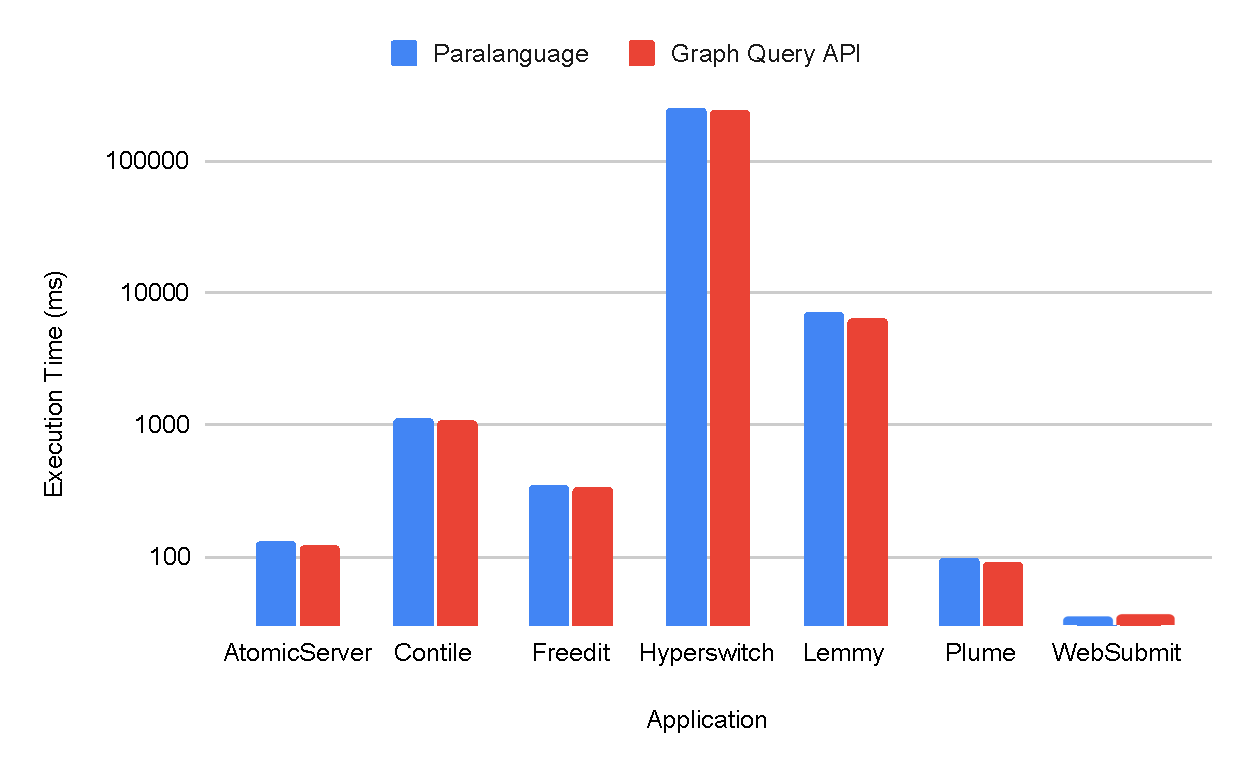
\includegraphics[scale=0.6]{graphics/times.pdf}
        \caption{
            \syslang{} and Graph Query policy execution times, on a logarithmic scale, averaged across 10 runs. 
            The \syslang{} execution times are similar to those of hand-optimized queries.
        }
        \label{f:times}
    \end{centering}
\end{figure}
%
\begin{figure}
    \small
    \begin{tabular}{|p{2.75cm}|p{2.75cm}|p{2.75cm}|p{2.75cm}|}
        \hline
        \textbf{Application} & \textbf{\syslang{} Time (ms)} & \textbf{Graph Query API Time (ms)} & \textbf{\syslang{} Percent Slower} \\ \hline
        AtomicServer & 127.92    & 118.8     & 7.68  \\ \hline
        Contile      & 1109.14   & 1064.43   & 4.2   \\ \hline
        Freedit      & 347.57    & 339.85    & 2.27  \\ \hline
        Hyperswitch  & 251044.37 & 241890.42 & 3.78  \\ \hline
        Lemmy        & 7026.23   & 6277.3    & 11.93 \\ \hline
        Plume        & 95.63     & 88.86     & 7.62  \\ \hline
        WebSubmit    & 29.89     & 30.07     & -0.6  \\ \hline               
        \end{tabular}
        \caption{
            Comparison of \syslang{} and Graph Query API policy execution times. 
            \syslang{} policies are, on average, marginally slower than the Graph Query API policies. 
        }
        \label{f:percentages}
\end{figure}

\section{Effort}
\label{sec:accessibility}

We evaluate the effort required to encode policies in \syslang{}.
%
Ideally, we would have conducted a user study with users unfamiliar with the system.
%
However, due to time limitations, we instead summarize our experience (as the authors of \sys{}) writing policies.
%

\paragraph{Policy Strictness:} We find that the effort required to encode policies in \syslang{} is proportional to the strictness of the policy.
%
For example, take the AtomicServer application, a graph-based database~\cite{atomic}.
%
A previous version of the application failed to verify that the 
user was permitted to modify a database resource before applying the update~\cite{atomic-fix}.
%
We encode this policy in \syslang{} by enforcing that if a database resource is modified,
the application checks which users are permitted to modify the resource,
and that check affects whether the update happens.
%
This policy fails on the buggy version of the application and passes on the fixed version.

Prior to this work, we wrote a version of this policy in the Graph Query API.
%
This policy was stricter: it also included the implementation-specific notion of \emph{commits}.
%
Commits are records of modifications to a resource (analogous to Git commits).
%
Our Graph Query API policy enforced that a commit had transitive data influence on the modified resource.
%
However, this assertion is not necessary to catch the permission check bug.
%

Throughout this work, we found multiple other instances where our \syslang{}
policies were simpler than the Graph API policies we wrote earlier.
%
Since the Graph Query API allows \devs{} access to the full expressive power of the PDG,
we often found ourselves referencing application source code to ensure that we selected the right primitives.
%
As a result, we unwittingly wrote policies that were more closely tied to the 
source code than actually necessary to express the policy we sought to check.
%
When we wrote the \syslang{} policies, 
we had a much smaller subset of predicates available.
%
We found that by abstracting away the full power of the PDG representation,
\syslang{} encouraged us to think about the minimum set of concepts
necessary to express our policies,
so our policies did not contain these unnecessary checks.

If a \ce{} does want to check in their \syslang{} policy that the modified resource is indeed
affiliated with a commit, they will need to expend more effort.
%
They may need to consult with the \dev{} to understand 
the implementation-specific notion of commits and how they interact with resources.
%
The \dev{} would also need to apply (and maintain) more markers to the application.

\paragraph{Numbered Clauses:} We found that for some of the policies, 
our first attempt to express them required more levels of numbered clauses than \sys{} supports~(\Cref{sec:other-limits}).
%
We refactored the policies to use definitions, 
which allowed us to express the policies with fewer nested expressions.
%
We found that this process made our final policies easier to read,
even if it took us longer to write them.